\documentclass[12pt, 
hyperref={colorlinks=true, linkcolor=blue, urlcolor=cyan},dvipsnames]{beamer}
\usetheme{default} 

\setbeamertemplate{navigation symbols}{} %gets rid of navigation symbols
\setbeamertemplate{footline}{} %gets rid of bottom navigation bars
\setbeamertemplate{footline}[page number]{} %use this for page numbers

\setbeamertemplate{itemize items}[circle] %round bullet points
\setlength\parskip{10pt} % white space between paragraphs

\usepackage{wrapfig}
\usepackage{subfig}
\usepackage{setspace}
\usepackage{enumerate}
\usepackage{graphicx}
\usepackage{amsmath}
\usepackage{amsfonts}
\usepackage{amssymb}
\usepackage{amsthm}
\usepackage{tikz}
\usepackage[UKenglish]{isodate}
\usepackage{xcolor}
\cleanlookdateon

% the preamble
\title{BIOST 311: \\ Regression Methods for the Health Sciences}
\author{Kelsey Grinde and Brian Williamson}
\institute{UW Biostatistics}
\date{Spring 2018}

\begin{document}
% title slide
\begin{frame}
\titlepage\thispagestyle{empty}
\end{frame}

% make it 4.something
\setbeamertemplate{footline}{%
  \raisebox{5pt}{\makebox[\paperwidth]{\makebox[120pt]{\scriptsize Last updated \today}\hfill\makebox[20pt]{\scriptsize 4.\insertframenumber~~}}}}  \newcounter{chap4}{\value{1}}
\setcounter{framenumber}{\value{chap4}}

\begin{frame}
\frametitle{CHAPTER 4: SPECIAL TOPICS}
At the end of this chapter, the typical student should be able to:
\begin{itemize}
\item describe why you might not want to use a parametric model,
\item describe a nonparametric statistical model,
\item describe a statistical parameter, 
\item and other things (TBD)
\end{itemize}
\end{frame}

\section{Nonparametric estimation and inference}
\begin{frame}
\frametitle{SECTION 1: {\small NONPARAMETRIC ESTIMATION AND INFERENCE}}
\framesubtitle{(by Brian)}

So far, in this course, you have explored how to answer scientific questions related to: \vspace{-0.3cm}
\begin{itemize}
\item causal associations,
\item associations (and prediction),
\item and effect modification,
\end{itemize} \vspace{-0.3cm}
using linear regression, logistic regression, or Cox proportional hazards regression.

You have also explored the necessary assumptions for these models to be valid.

Fundamentally, however, these tools \textcolor{red}{all make potentially restrictive assumptions} on the true data-generating mechanism (i.e., the process that truly creates the data as we see it).
\end{frame}

% introduce the variable importance problem, in the context of HIV vaccine
\begin{frame}
\frametitle{Case study: variable importance}
A new frontier in HIV-1 vaccine research studies \textcolor{blue}{broadly neutralizing antibodies}: HIV-1 is diverse and mutates quickly, so successful antibodies against HIV-1 must be able to recognize and neutralize many strains. \pause

VRC01: \vspace{-0.3cm}
\begin{itemize}
\item a broadly neutralizing antibody against HIV-1
\item isolated from a donor chronically infected with HIV-1 for 15 years
\item neutralizes over 80\% of $> 600$ viral strains tested
\end{itemize} \pause

The Antibody Mediated Prevention (AMP) trials, expected to finish in 2020, \textcolor{blue}{assess the efficacy of VRC01 in preventing HIV-1 infection}.
\end{frame}

% variable importance
\begin{frame}
\frametitle{Case study: variable importance}
Part of the pre-planned analysis of these data involves testing those viruses that do cause infection, even in the presence of VRC01.

\textcolor{blue}{Differences in prevention efficacy based on features of these viruses give us information about how VRC01 works to prevent infection}, and give us \textcolor{ForestGreen}{clues about how to develop an effective vaccine.} \pause

I am primarily interested in features of the HIV-1 genotype, but there are \textcolor{red}{many ways} to define an HIV-1 genotype; this implies that \textcolor{red}{if we test each amino acid (AA) feature, and apply a multiple comparisons correction, it will be difficult to detect effects. }
\end{frame}

% variable importance!
\begin{frame}
\frametitle{Case study: variable importance}
Fortunately, there are publicly available data on the neutralization sensitivity of HIV-1 viruses to VRC01. I am currently collaborating with researchers at the Fred Hutchinson Cancer Research Center to:
\begin{itemize}
\item develop an algorithm with \textcolor{ForestGreen}{good accuracy in predicting neutralization sensitivity} from HIV-1 AA features, and
\item \textcolor{blue}{rank AA features by their importance in predicting neutralization sensitivity}, and advance the top ranked features to the AMP analysis
\end{itemize}

Fitting \textcolor{ForestGreen}{complex machine learning-based methods} achieves the first objective; the second objective is a \textcolor{blue}{bit more nuanced}.
\end{frame}

\begin{frame}
\frametitle{Common data analysis goals}
\begin{center}
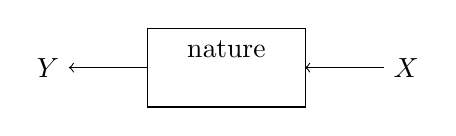
\begin{tikzpicture}
\node [left] at (0,1) {$Y$};
\node [right] at (4, 1) {$X$};
\draw [fill=white] (1,0.5) rectangle (3,1.5);
\node [above] at (2,1) {nature};
\draw [<-] (3,1) -- (4,1);
\draw [<-] (0,1) -- (1,1);
\end{tikzpicture}
\end{center}

Goals: \vspace{-0.3cm}
\begin{itemize}
\item Extract some information about the \textcolor{blue}{\textit{association}} between response and predictors in nature
\item \textcolor{blue}{\textit{Predict}} what the response will be with future predictors
\end{itemize} 
\end{frame}

% models, as you have seen them
\begin{frame}
\frametitle{Statistical models, as you have seen them}
Examples of statistical models: \vspace{6cm}
\end{frame}

\begin{frame}
\frametitle{Statistical models, as you have seen them}
Often, we use a \textcolor{red}{parametric model} for the relationship between our predictors and the response, for example: \vspace{-0.3cm}
\begin{itemize}
\item $Y \sim Bernoulli(p)$ 
\item $Y \sim N(0, 1)$
\item $E(Y \mid X) = \beta_0 + \beta_1 X$ 
\item $\text{logit} \{E(Y \mid X)\} = \beta_0 + \beta_1 X$
\end{itemize}

In the first two cases, \textcolor{magenta}{knowledge of a finite number of population parameters determines the entire distribution.}

In the second two cases, \textcolor{olive}{we specify (some function of) the conditional expectation as a linear function of a finite number of population parameters.}
\end{frame}

\begin{frame}
\frametitle{Statistical models, as you have seen them}
Advantages to a finite parametric model: \vspace{-0.3cm}
\begin{itemize}
\item \textcolor{blue}{simple} (too complex can be bad)
\item \textcolor{Aquamarine}{convenient} (we know how to fit them)
\end{itemize}

\end{frame}

\begin{frame}
\frametitle{Statistical models, as you have seen them}
Disadvantages to a finite parametric model: \vspace{-0.3cm}
\begin{itemize}
\item often, \textcolor{red}{the type of data at hand (rather than the scientific question) dictates the model used}, and parameters of interest are then determined by default:
\begin{itemize}
\item continuous outcome $+$ covariates $\rightarrow$ linear regression
\item binary outcome $+$ covariates $\rightarrow$ logistic regression
\item survival outcome $+$ covariates $\rightarrow$ proportional hazards regression
\end{itemize}
\item \textcolor{olive}{do we really care about these parameters?}
\item \textcolor{magenta}{what happens if the model is misspecified?}
\begin{itemize}
\item what are we estimating?
\item is inference valid for what we are actually estimating?
\end{itemize}
\end{itemize}
\end{frame}

% parameters, as you have seen them
\begin{frame}
\frametitle{Statistical parameters, as you have seen them}

\textcolor{magenta}{The parameters of interest define, or index, the model:} \vspace{-0.3cm}
\begin{itemize}
\item $p$ defines a $Bernoulli(p)$
\item[]
\item[]
\item $(\mu, \sigma)$ defines a $N(\mu, \sigma^2)$
\item[]
\item[]
\item $\beta_0, \beta_1$ define a simple regression model
\item[]
\item[]
\end{itemize}

\end{frame}

% breiman "modeling"
\begin{frame}
\frametitle{Common current approaches to modeling}
\begin{center}
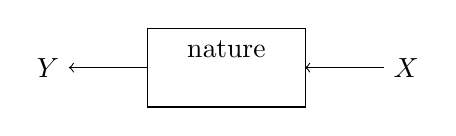
\begin{tikzpicture}
\node [left] at (0,1) {$Y$};
\node [right] at (4, 1) {$X$};
\draw [fill=white] (1,0.5) rectangle (3,1.5);
\node [above] at (2,1) {nature};
\draw [<-] (3,1) -- (4,1);
\draw [<-] (0,1) -- (1,1);
\end{tikzpicture}
\end{center} \pause

Traditional statistical modeling:
\begin{center}
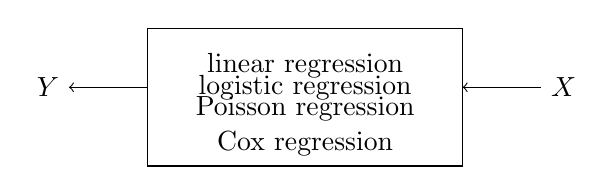
\begin{tikzpicture}
\node [left] at (0,1) {$Y$};
\node [right] at (6, 1) {$X$};
\draw [fill=white] (1,0) rectangle (5,1.75);
\node [above] at (3,1) {linear regression};
\node at (3,1) {logistic regression};
\node [below] at (3,1) {Poisson regression};
\node [above] at (3,0) {Cox regression};
\draw [<-] (5,1) -- (6,1);
\draw [<-] (0,1) -- (1,1);
\end{tikzpicture}
\end{center} \pause

Algorithmic modeling:

\begin{center}
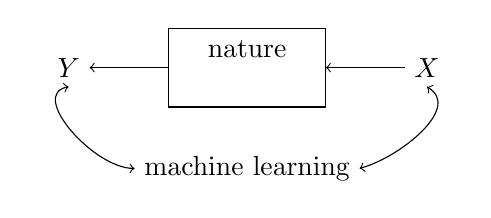
\begin{tikzpicture}
\node [left] (1) at (0,1) {$Y$};
\node [right] (2) at (4, 1) {$X$};
\draw [fill=white] (1,0.5) rectangle (3,1.5);
\node [above] at (2,1) {nature};
\draw [<-] (3,1) -- (4,1);
\draw [<-] (0,1) -- (1,1);
\node [below] (3) at (2,0) {machine learning};
\draw [<->] (2.south) to [out = -30, in = 15] (3.east);
\draw [<->] (1.south) to [out = 190, in = 180] (3.west);
\end{tikzpicture}
\end{center}
\end{frame}

% models, as I see them
\begin{frame}
\frametitle{Statistical models, as I see them}
Fundamentally, \textcolor{blue}{statistical models are collections of plausible probability distributions, and need not be indexed by a finite-dimensional parameter.}

We should \textcolor{blue}{put as much knowledge as possible into choosing this model}, \textcolor{ForestGreen}{but make sure that the true data-generating mechanism will be contained in it.} This is where we ``model'' nature!
\begin{center}
\begin{tikzpicture}
\draw (0,0) ellipse (2.5cm and 2cm);
\node [below] at (1,-1) {$\mathcal{M}$}; 
\draw [fill] (-1, 1) circle [radius=0.05];
\node [right] at (-1,1) {$P_0$};
\end{tikzpicture}
\end{center}
\end{frame}

% parameters, as I see them
\begin{frame}
\frametitle{Statistical parameters, as I see them}
A \textbf{finite-dimensional parameter} takes as input a probability distribution, and outputs a real number (or a vector). \vspace{-0.3cm}
\begin{itemize}
\item[] e.g.: mean, variance, correlation, $\dots$
\end{itemize} \pause

\begin{center}
\begin{tikzpicture}
\draw (0,0) ellipse (2.5cm and 2cm);
\node [below] at (1,-1) {$\mathcal{M}$}; 
\draw [fill] (-1, 1) circle [radius=0.05];
\node [right] at (-1,1) {$P_0$};
\draw [<->] (4, 0.5) -- (8, 0.5);
\draw[fill] (0,0) circle [radius=0.05];
\node [above] (0, 0) {$P$};
\draw [->] (0,0) to [out = -30, in = -90] (7, 0.5) node [above] {$\Psi(P)$};
\draw [fill] (7, 0.5) circle [radius = 0.05];
\node [below] at (4, -1.5) {$\Psi$};
\end{tikzpicture}
\end{center} \pause

Our goal, typically, is to estimate the \textbf{true parameter value} $\psi_0 := \Psi(P_0)$ based on observations drawn from $P_0$.
\end{frame}

\begin{frame}
\frametitle{Statistical parameters, as I see them}
\begin{center}
\begin{tikzpicture}
\draw (0,0) ellipse (2.5cm and 2cm);
\node [below] at (1,-1) {$\mathcal{M}$}; 
\draw [fill] (-1, 1) circle [radius=0.05];
\node [right] at (-1,1) {$P_0$};
\draw [<->] (4, 0.5) -- (8, 0.5);
\draw[fill] (0,0) circle [radius=0.05];
\node [above] (0, 0) {$P$};
\draw [->] (0,0) to [out = -30, in = -90] (7, 0.5) node [above] {$\Psi(P)$};
\draw [fill] (7, 0.5) circle [radius = 0.05];
\node [below] at (4, -1.5) {$\Psi$};
\end{tikzpicture}
\end{center}

$\mathcal{M}$ \textcolor{ForestGreen}{encodes our knowledge about nature.} \pause

$P_0$ \textcolor{cyan}{is the true data-generating mechanism (unknown).} \pause

$\Psi$ \textcolor{blue}{tells us about nature, and is something we can estimate.}
\end{frame}

% modeling culture
\begin{frame}
\frametitle{My modeling approach}
\textcolor{blue}{Writing the statistical model and parameter separately allow us to disentangle the parameter and estimation.}

Proposed workflow:
\begin{enumerate}
\item Define a statistical model (often nonparametric, or not indexed by a finite-dimensional parameter) \pause
\item Define statistical parameter of interest \pause
\item Choose an estimation procedure for this parameter
\end{enumerate} \pause

However, steps 2 and 3 involve work: once a useful parameter is defined, it must be studied so that we can estimate it unbiasedly and obtain valid inference for it.
\end{frame}

% how would we address this using linear regression?
\begin{frame}
\frametitle{Case study: variable importance}
Variable importance in linear regression: e.g., $E(Y \mid X_1, X_2) = \beta_0 + \beta_1 X_1 + \beta_2 X_2$ \pause
\begin{itemize}
\item $\beta_1$: difference in mean $Y$ for two groups differing by one unit in $X_1$, with the same value of $X_2$ \pause
\item $X_1$ has no effect on $Y$ if $\beta_1 = 0$ (i.e., is unimportant) \pause
\item estimate importance (i.e., deviation from the null) with $\lvert (\hat{\beta}_1 - 0)/SE(\hat{\beta}_1) \rvert$ \pause
\end{itemize}

However, it is possible that our variables of interest are important in other ways besides the linear association. If the linear model doesn't hold, \textcolor{red}{then these variable importance estimates are meaningless.}
\end{frame}


% variable importance parameter
\begin{frame}
\frametitle{Case study: variable importance}
In this context, we define variable importance using a nonparametric extension of $R^2$ variable importance (see 1.164--1.165):
\begin{align*}
\Psi_s(P) = &\ \frac{\int \{E_P(Y \mid X) - E_P(Y \mid X_{(-s)})\}^2 dP(x)}{var_P(Y)}
\end{align*}

\textcolor{cyan}{This measures the additional proportion of the variability in the outcome explained by including the features $X_s$ in the regression} ($s$ can index a single feature or group of features). \pause

\textcolor{red}{Coming up with a parameter can be hard work:} this particular parameter resulted from multiple consultations between statisticians and epidemiologists.

However, this work is worth it: at the end of the day, you are estimating something you care about!
\end{frame}

% how to estimate it?
\begin{frame}
\frametitle{Case study: variable importance}
\vspace{-0.75cm}
\begin{align*}
\Psi_s(P) = &\ \frac{\int \{E_P(Y \mid X) - E_P(Y \mid X_{(-s)})\}^2 dP(x)}{var_P(Y)}
\end{align*}
\vspace{-0.4cm}
I need to estimate four objects:
\begin{itemize}
\item the probability distribution of the $X$ data \pause
\item the conditional expectation given $X$ \pause
\item the conditional expectation given $X_{(-s)}$ \pause
\item the variance of $Y$ \pause
\end{itemize}

\textcolor{blue}{The first and last components are easy}: take the empirical variance, and take a simple average once I have the middle two components. \pause

\textcolor{red}{The middle two components are where I can run into trouble if I make incorrect assumptions. }
\end{frame}

% ML tools
\begin{frame}
\frametitle{Estimating a conditional mean}
So far, this quarter, we have studied four methods for estimating conditional means (also called \textcolor{blue}{regression functions}):
\begin{itemize}
\item linear regression,
\item logistic regression, 
\item Poisson regression, and
\item Cox proportional hazards regression.
\end{itemize}

Each of these tools makes the fundamental assumption that some function of the conditional mean is linear in the model parameters, which is \textcolor{red}{potentially quite restrictive}. 

More model-agnostic regression techniques are known colloquially as ``machine learning'' tools.
\end{frame}

% the bias-variance tradeoff
\begin{frame}
\frametitle{Estimating a conditional mean}
Typically, machine learning-based methods involve some sort of \textcolor{ForestGreen}{bias-variance tradeoff} (see slides 1.168--1.170): the idea is to \textcolor{red}{increase bias} a bit for \textcolor{blue}{decreased variance}, and possibly better predictions. \pause

This means that, in particular, \textbf{inference based on machine learning techniques is difficult}; the added bias is often difficult to characterize, and classical statistical results (like the Central Limit Theorem) do not apply, in general. \pause

Many machine learning-based methods are implemented in \texttt{R}, and many of them use the same notation we have used throughout the quarter: \texttt{Y} $\sim$ \texttt{X\_1 + X\_2 + \dots}

\end{frame}

\begin{frame}
\frametitle{Estimating a conditional mean}
You can already use one particular kind of machine learning algorithm, called \textbf{model stacking}. Here, we 
\begin{enumerate}
\item fit many types of regression (or other algorithm)
\item average the fitted values from (1), yielding a final set of fitted values
\end{enumerate}
This removes some subjectivity from the process, and means that \textcolor{blue}{the more different algorithms we use, the more robust our results are to potential misspecification of one algorithm!}
\end{frame}

\begin{frame}
\frametitle{Inference when using machine learning techniques}

However, typically the bias-variance tradeoff we make for estimating the conditional mean is \textbf{not} the optimal bias-variance tradeoff for estimating our parameter of interest (e.g., variable importance).

A large part of my research is focused on characterizing the properties of the parameter of interest, so that we can \textcolor{blue}{correct} for this non-optimal bias-variance tradeoff.

At the end of the day, if I have done my job correctly, we have an estimator of the parameter of interest that has an asymptotic normal distribution by the Central Limit Theorem (just like our regression estimators!).

In particular, this means that \textcolor{blue}{we can create confidence intervals and do hypothesis tests}, even though we have used flexible methods in estimation.
\end{frame}

\begin{frame}
\frametitle{Nonparametric estimation and inference: summary}

\textcolor{red}{Parametric models are potentially quite restrictive, and may lead us astray if the model is misspecified}. We often have no way of verifying if the model holds or not! \pause

\textcolor{ForestGreen}{Machine learning techniques offer a flexible alternative}: rather than specifying a model, we let the data tell us what the conditional mean looks like. \pause

However, \textcolor{Aquamarine}{we lose interpretability if we only use machine learning-based methods}. \pause

Doing the work to define and understand the properties of \textbf{statistical parameters} can help here: \textcolor{blue}{we can use machine learning tools as an intermediate step to flexibly estimate a parameter of interest, and still develop confidence intervals and do hypothesis tests! }
\end{frame}

\section{Statistical genetics}
\begin{frame}
\frametitle{SECTION 2: {\small REGRESSION IN STATISTICAL GENETICS}}
\framesubtitle{(by Kelsey)}

Learning Objectives:
\begin{itemize}
\item Write down a regression model for a genetic association study (GWAS or admixture mapping)
\item Interpret results from a genetic association study (GWAS or admixture mapping)
\item Explain why we can't use the p-value threshold 0.05 in GWAS or genome-wide admixture mapping studies to declare results ``statistically significant"
\end{itemize}

\end{frame}

\begin{frame}
\frametitle{Quick Detour: Project Presentations}

\begin{itemize}
\item We \textbf{will not} be evaluating your presentation or slide-making skills! (audience = classmates, not us)
\item Share talking time equally among group members
\item You have 10 minutes (including questions); goal = 8
\item You can use up to 8 slides, but you only need 6:
	\begin{enumerate}
	\item Background
	\item Scientific question (just pick one!)
	\item What did you do? (descriptives, regression model)
	\item What did you find? (plot or numerical summaries)
	\item What did you find? (regression results)
	\item Discussion (summary, implications, challenges)
	\end{enumerate}
\item Save slides as PDF, upload to Canvas by 10am Tues
\item You'll present in order of Group \#'s 
\end{itemize}

\end{frame}

% motivating examples
\begin{frame}
\frametitle{Motivating Examples}

\textbf{Statistical genetics:} ``develop statistical methods for understanding the genetic basis of human diseases and traits"\footnote[frame]{https://www.hsph.harvard.edu/statistical-genetics/} \pause

``Success" stories:\vspace{-0.3cm} 
\begin{itemize}
\item Huntington's disease and the \textit{Huntingtin} gene \pause
\item \textit{\href{https://www.nytimes.com/2013/05/14/opinion/my-medical-choice.html}{BRCA1}, BRCA2} and breast cancer \pause
\item \href{https://www.nature.com/articles/ncomms10448}{Are you a morning person?} (23andMe) \pause
\item \href{https://www.soccergenomics.com/}{Soccer genomics}
\end{itemize}
\end{frame}

% regression model for Y ~ genotype
\begin{frame}
\frametitle{Genetic Association Studies: Regression Models}

\textbf{Scientific Question:} is gene $X$ associated with trait $Y$?

\begin{itemize}
\item[] We often look at the genotype (GG GA AA)
\end{itemize} \pause

\textcolor{blue}{Activity:} write down a linear regression model that we could use to answer this scientific question.

\end{frame}

% interpreting GWAS results
\begin{frame}
\frametitle{Genetic Association Studies: Interpretation}

$$E[\text{Height (inches)} \mid \text{Number of A's}] = \beta_0 + \beta_1 \text{Number of A's}$$

\textcolor{blue}{Activity:} interpret the coefficient estimate $\hat\beta_1 = 0.1$ \pause

\hspace*{-1cm}
\includegraphics[width=1.17\textwidth]{figs/23andMe_interp}

What do you think of the interpretation from 23andMe?

\end{frame}

% intro to GWAS, motivate multiple testing problem
\begin{frame}
\frametitle{Genome-Wide Association Studies (GWAS)}

$$E[Y \mid \# \text{``rare" alleles at loc } j] = \beta_0 + \beta_{1,j} \left(\# \text{``rare" alleles at loc } j\right)$$ \textbf{GWAS:} repeat for all locations across the genome $j = 1, ..., m$ \pause

\begin{columns}
\begin{column}{0.7\textwidth}
\begin{itemize}
\item In entire genome: $m \approx 3$ billion
\item In most GWAS: thousands or millions
\end{itemize}
\end{column}

\begin{column}{0.3\textwidth}
\vspace{0.3cm}
\includegraphics[angle=270,origin=c,width=\textwidth]{figs/bookcase}
\end{column}
\end{columns}

\end{frame}

\begin{frame}
\frametitle{GWAS: Multiple Testing}
\begin{itemize}
\item What happens if we use the significance threshold 0.05? \pause
	\begin{itemize}
	\item 1 test: 5\% chance of type I error \begin{footnotesize}(incorrectly reject $H_0$) \end{footnotesize} \pause
	\item 100 tests: expect to see 5 type I errors \pause
	\item 1 million tests: expect to see ??? type I errors \pause
	\end{itemize}
\item What do we use instead? \pause \textcolor{red}{Bonferroni correction} 
\end{itemize}

\includegraphics[width=\textwidth]{figs/morning_manhattan}

\end{frame}

% intro to admixture mapping
\begin{frame}
\frametitle{Intro to Admixture Mapping}

[overall goal]

[how is it different from GWAS?]

\end{frame}

\begin{frame}
\frametitle{Quick Detour: Ancestry Inference}

[My 23andMe results]

\end{frame}


\begin{frame}
\frametitle{Admixture Mapping: Regression Models}

\textbf{Scientific Question:} is ancestry at locus $j$ associated with trait $Y$?

[Include picture with $K=3$ from general exam slides]

\textcolor{blue}{Activity:} write down a linear regression model that we could use to answer this scientific question.

\end{frame}

\begin{frame}
\frametitle{Admixture Mapping: Multiple Testing}

[The topic of my dissertation!]

\end{frame}



% Minute Paper
\begin{frame}
\frametitle{Index Card: Reflection}

Please answer the following questions:
\begin{enumerate}
\item List something you've learned in this course (even better if it's something you're excited to have learned)
\item List something you're still confused about and/or want to understand better before the end of the quarter
\item If we held office hours during finals week, would you attend?
	\begin{enumerate}
	\item If yes, does Wednesday 2--4pm work for you? (Otherwise, please suggest a couple times that work better.)
	\end{enumerate}
\end{enumerate}

\textcolor{blue}{Don't forget to complete the course evaluations by June 1!}

\end{frame}


\section{Correlated data}

\end{document}
